%% BioMed_Central_Tex_Template_v1.06
%%                                      %
%  bmc_article.tex            ver: 1.06 %
%                                       %

%%IMPORTANT: do not delete the first line of this template
%%It must be present to enable the BMC Submission system to
%%recognise this template!!

%%%%%%%%%%%%%%%%%%%%%%%%%%%%%%%%%%%%%%%%%
%%                                     %%
%%  LaTeX template for BioMed Central  %%
%%     journal article submissions     %%
%%                                     %%
%%          <8 June 2012>              %%
%%                                     %%
%%                                     %%
%%%%%%%%%%%%%%%%%%%%%%%%%%%%%%%%%%%%%%%%%

%%%%%%%%%%%%%%%%%%%%%%%%%%%%%%%%%%%%%%%%%%%%%%%%%%%%%%%%%%%%%%%%%%%%%
%%                                                                 %%
%% For instructions on how to fill out this Tex template           %%
%% document please refer to Readme.html and the instructions for   %%
%% authors page on the biomed central website                      %%
%% https://www.biomedcentral.com/getpublished                      %%
%%                                                                 %%
%% Please do not use \input{...} to include other tex files.       %%
%% Submit your LaTeX manuscript as one .tex document.              %%
%%                                                                 %%
%% All additional figures and files should be attached             %%
%% separately and not embedded in the \TeX\ document itself.       %%
%%                                                                 %%
%% BioMed Central currently use the MikTex distribution of         %%
%% TeX for Windows) of TeX and LaTeX.  This is available from      %%
%% https://miktex.org/                                             %%
%%                                                                 %%
%%%%%%%%%%%%%%%%%%%%%%%%%%%%%%%%%%%%%%%%%%%%%%%%%%%%%%%%%%%%%%%%%%%%%

%%% additional documentclass options:
%  [doublespacing]
%  [linenumbers]   - put the line numbers on margins

%%% loading packages, author definitions

%\documentclass[twocolumn]{bmcart}% uncomment this for twocolumn layout and comment line below
\documentclass{bmcart}

%%% Load packages
\usepackage{amsthm,amsmath}
%\RequirePackage[numbers]{natbib}
%\RequirePackage[authoryear]{natbib}% uncomment this for author-year bibliography
%\RequirePackage{hyperref}
\usepackage[utf8]{inputenc} %unicode support
%\usepackage[applemac]{inputenc} %applemac support if unicode package fails
%\usepackage[latin1]{inputenc} %UNIX support if unicode package fails

%for abbreviations item list
\usepackage{blindtext}
\usepackage{enumitem}
\usepackage{xcolor}
%for url
%\usepackage{hyperref}
%
%include figure 
\usepackage{graphicx}

%%%%%%%%%%%%%%%%%%%%%%%%%%%%%%%%%%%%%%%%%%%%%%%%%
%%                                             %%
%%  If you wish to display your graphics for   %%
%%  your own use using includegraphic or       %%
%%  includegraphics, then comment out the      %%
%%  following two lines of code.               %%
%%  NB: These line *must* be included when     %%
%%  submitting to BMC.                         %%
%%  All figure files must be submitted as      %%
%%  separate graphics through the BMC          %%
%%  submission process, not included in the    %%
%%  submitted article.                         %%
%%                                             %%
%%%%%%%%%%%%%%%%%%%%%%%%%%%%%%%%%%%%%%%%%%%%%%%%%


%\def\includegraphic{}
%\def\includegraphics{}

%%% Put your definitions there:
\startlocaldefs
\endlocaldefs

\usepackage{xcolor}
\newcommand{\comment}[1]{ \color{red} #1 \color{black}}
\newcommand{\reply}[1]{ \color{blue} [#1] \color{black}}
\newcommand{\revision}[1]{ \color{blue} [#1] \color{black}}
\newcommand{\eqn}[1]{Eq.~(\ref{#1})}
\newcommand{\fig}[1]{Fig.~\ref{#1}}
\newcommand{\tab}[1]{Table~\ref{#1}}
\newcommand{\sect}[1]{Section~\ref{#1}}

%%% Begin ...
\begin{document}

%%% Start of article front matter
%\begin{frontmatter}

%\begin{fmbox}

%\dochead{Research}

%%%%%%%%%%%%%%%%%%%%%%%%%%%%%%%%%%%%%%%%%%%%%%
%%                                          %%
%% Enter the title of your article here     %%
%%                                          %%
%%%%%%%%%%%%%%%%%%%%%%%%%%%%%%%%%%%%%%%%%%%%%%
\raggedright
{\Large An Oscillating Reaction Network With an Exact Closed-Form Time-Domain Solution:
Solution Derivation}
\vskip .2cm
{\large Joseph L. Hellerstein}
\linebreak
eScience Institute
\linebreak
University of Washington
\linebreak
Seatttle, Washington

%%%%%%%%%%%%%%%%%%%%%%%%%%%%%%%%%%%%%%%%%%%%%%
%%                                          %%
%% Enter the authors here                   %%
%%                                          %%
%% Specify information, if available,       %%
%% in the form:                             %%
%%   <key>={<id1>,<id2>}                    %%
%%   <key>=                                 %%
%% Comment or delete the keys which are     %%
%% not used. Repeat \author command as much %%
%% as required.                             %%
%%                                          %%
%%%%%%%%%%%%%%%%%%%%%%%%%%%%%%%%%%%%%%%%%%%%%%

%\author[
%  addressref={aff1},                   % id's of address
%  corref={aff1},
%  email={jlheller@uw.edu}
  %{aff1,aff2}
% corref={aff1},                       % id of corresponding %address, if any
% noteref={n1},                        % id's of article notes, %if any
%  email={jane.e.doe@cambridge.co.uk}   % email address
%]{\inits{J.L.H.}\fnm{Joseph} \snm{Hellerstein}}
%\author[
%  addressref={aff1},                   % id's of address
%]{\inits{H.M.S.}\fnm{Herbert M.} \snm{Sauro}}
%\author[
%  addressref={aff2},
  %corref={aff2},
  %email={joseph.hellerstein@gmail.com}
%]{\inits{J.H.}\fnm{Joseph L.} \snm{Hellerstein}}

%%%%%%%%%%%%%%%%%%%%%%%%%%%%%%%%%%%%%%%%%%%%%%
%%                                          %%
%% Enter the authors' addresses here        %%
%%                                          %%
%% Repeat \address commands as much as      %%
%% required.                                %%
%%                                          %%
%%%%%%%%%%%%%%%%%%%%%%%%%%%%%%%%%%%%%%%%%%%%%%
%\address[id=aff2]{%
%  \orgdiv{eScience Institute},
%  \orgname{University of Washington},
%  %\street{},
%  %\postcode{}
%  \city{Seattle},
%  \cny{USA}
%}

%%%%%%%%%%%%%%%%%%%%%%%%%%%%%%%%%%%%%%%%%%%%%%
%%                                          %%
%% Enter short notes here                   %%
%%                                          %%
%% Short notes will be after addresses      %%
%% on first page.                           %%
%%                                          %%
%%%%%%%%%%%%%%%%%%%%%%%%%%%%%%%%%%%%%%%%%%%%%%

%\begin{artnotes}
%%\note{Sample of title note}     % note to the article
%\note[id=n1]{Equal contributor} % note, connected to author
%\end{artnotes}

%\end{fmbox}% comment this for two column layout
%\end{frontmatter}

%%%%%%%%%%%%%%%%%%%%%%%%%%%%%%%%%%%%%%%%%%%%%%%
%%                                           %%
%% The Abstract begins here                  %%
%%                                           %%
%% Please refer to the Instructions for      %%
%% authors on https://www.biomedcentral.com/ %%
%% and include the section headings          %%
%% accordingly for your article type.        %%
%%                                           %%
%%%%%%%%%%%%%%%%%%%%%%%%%%%%%%%%%%%%%%%%%%%%%%%
\setlength{\parindent}{15pt}

%%%%%%%%%%%%%%%%%%%%%%%%%%%%%%%%%%%
\section{Preliminaries}

%%%%%%%%%%%%%%% reaction-network
This write-up provides details on the derivation of the
time domain solution for the
reaction network depicted in Fig.~\ref{fig:reaction-network}.
Recall that the reaction network is constructed so that its kinetics are described by a system of linear ODEs with sustained oscillations.
The time domain solution is an initial value problem (IVP).

\par
The reaction network has 8 parameters. There are 6 kinetic constants,
$k_i,~ i\in \{1, 2, 3, 4, 5, 6\}$. And there are two initial
concentrations, $x_n (0),~ n \in \{1, 2 \}$, where $x_n(0)$ is the
initial concentration for $S_n$.

Because the dynamics of the network can be described by an oscillating linear system, we
know that oscillations are sinusoids.
Let $x_n (t)$ be the concentration
of species $S_n$ at time $t$. Then, an oscillating solution has the
form \begin{equation*}
x_n(t) = \alpha_n sin(\theta_n t + \phi_n) + \omega_n,
\end{equation*} where $\alpha_n$ is the amplitude of the sinusoid for
$S_n$, $\theta_n$ is its frequency, $\phi_n$ is its phase, and
$\omega_n$ is the DC offset (the mean value of the sinusoid over
time).
As we show shortly, both species have the same frequency.
So, $\theta_n = \theta$, and there are just 7 parameters.
We refer to $\alpha_n, \theta, \phi_n, \omega_n$ as the
\textbf{oscillation characteristics (OC)} of the reaction network.

We make use of the vector representation of linear systems of ODEs.
\begin{equation*}
\dot{\bf x} = {\bf A} {\bf x} + {\bf u}
\end{equation*} where the Jacobian matrix is
${\bf A} = \begin{pmatrix} a_{11} & a_{12} \\ a_{21} & a_{22} \\ \end{pmatrix}$,
${\bf x} (t)$ is the state vector,
$\dot {\bf x} (t)$ is the time derivative of the state vector, and ${\bf u}$ is the time-independent forced inputs.

\begin{figure}
        \centering
         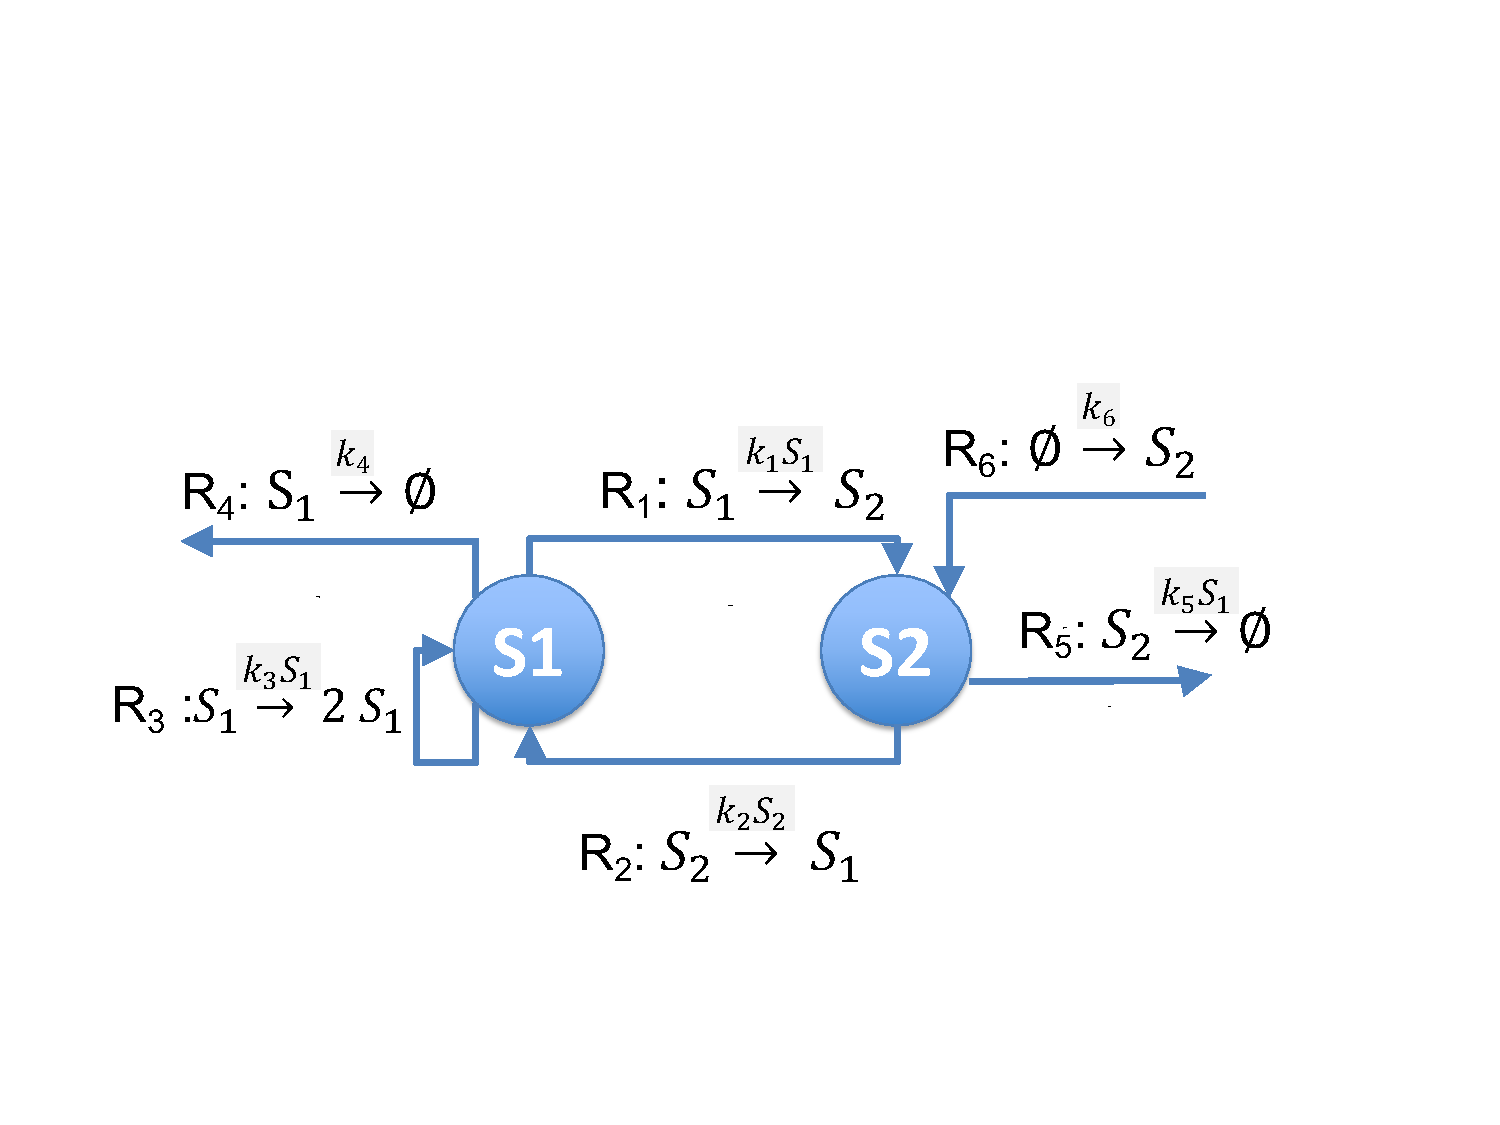
\includegraphics[scale=0.5]{Fig1.pdf}
         \caption[]{Reaction network that creates oscillations in the chemical species $S_1, S_2$. The reaction network is designed so that its time domain solution is a system of linear differential equations. The text describes constraints on the kinetic constants ($k_i$) and initial conditions of the chemical species to create an oscillator such that species concentrations are non-negative, a requirement for biological feasibility.}
         \label{fig:reaction-network}
\end{figure}

%%%%%%%%%%%%%%%%%%%%%%%%%%%%%%%%%%%
\section{Jacobian and Eigenvalues}
Here, we construct the Jacobian of the reaction network, and calculate its eigenvalues.

If there is an oscillating solution for this system, then the
eigenvalues of ${\bf A}$ must be pure imaginary. Since this is a two
state system, this means that if $\theta i$ is an eigenvalue, then
$-\theta i$ must also be an eigenvalue. This means that
$\theta_1 = \theta = \theta_2$, which justifies our previous claim that the two species have the same oscillation frequency.

Next we develop the conditions for the Jacobian
${\bf A}$ to have a pure imaginary
eigenvalues. The determinant of ${\bf A}$ is
$det({\bf A}) = a_{11} a_{22} - a_{12} a_{21} = \Delta.$
The trace of
${\bf A}$ is $tr({\bf A}) = a_{11} + a_{22} = \tau.$
So, the eigenvalues $\lambda_n$ are
$\frac{1}{2} \left( - \tau \pm \sqrt{\tau^2 - 4 \Delta} \right). $
We get pure imaginary eigenvalues 
if the following constraints hold:
\begin{itemize}
\item $\tau = 0$ 
\item $\Delta > 0.$
\end{itemize}

For the reaction network, ${\bf A}$ is
\begin{equation*}
{\bf A} =
\begin{pmatrix}
k_3 - k_1 & k_2 \\
k_1 - k_5 & -k_2 \\
\end{pmatrix}
\end{equation*}

and 
\begin{equation*}
{\bf u} = 
\begin{pmatrix} - k_4 \\ k_6 \\ \end{pmatrix}
\end{equation*}
So the trace and determinant are:
\begin{eqnarray*}
\tau & = & k_3 -k_1 - k_2 \\
\Delta & = & (k_3 - k_1)(-k_2) - k_2 (k_1 - k_5) \\
& = & k_2 (k_5 - k_3) \\
\end{eqnarray*}

$\tau = 0$ implies that $k_3 = k_1 + k_2$. $\Delta > 0$
implies that that $k_5 > k_3$. We define $k_d = k_5 - k_3 > 0$
Applying the foregoing to the ${\bf A}$ matrix, we first note that
\begin{align*}
k_1 - k_5 & = & k_1 - k_3 -k_d \\
& = & k_3 - k_2 - k_3 - k_d \\
& = & -k_2 - k_d \\
\end{align*}
Applying the constraints,
we see that
\begin{equation*}
{\bf A} = 
\begin{pmatrix}
k_2 & k_2 \\
-k_2 - k_d & -k_2 \\
\end{pmatrix}
\end{equation*}
Observe that $\Delta = k_2 k_d$.
As a result
$\theta = \pm \sqrt{\Delta} = \pm \sqrt{k_2 k_d}$. The negative sign affects phase, not frequency; we address phase separately. So, hereafter, we drop
the $\pm$.

%%%%%%%%%%%%%%%%%%%%%%%%
\section{Eigenvectors and Fundamental Matrix}

We find the eigenvectors of ${\bf A}$ as an intermediate step to
solving the IVP.

First, observe that that since $k_d > 0$, ${\bf A}$ is nonsingular,
and so we can calculate eigenvectors directly.

\begin{equation*}
    {\bf w}_1 =
    \begin{pmatrix}
- \frac{k_{2}}{k_{2} + k_{d}}
+ \frac{i \theta}{k_{2} + k_{d}} 
\\ 1
\end{pmatrix}
\end{equation*}
for the eigenvalue $\lambda_1 = - \sqrt{k_d k_2}$.

\begin{equation*}
    {\bf w}_2 =
    \begin{pmatrix}
- \frac{k_{2}}{k_{2} + k_{d}}
- \frac{i \theta}{k_{2} + k_{d}} 
\\ 1
\end{pmatrix}
\end{equation*}
for the eigenvalue $\lambda_1 = \sqrt{k_d k_2}$.

The {\bf fundamental matrix} {\bf F} of a system of 
linear ODEs has a column
for each
${\bf w}_n e^{\lambda_n}$.
Rather than writing ${\bf F} (t)$ immediately, we first
observe that it can be transformed into
a real valued matrix. This involves factoring the
eigenvectors into
real and imaginary parts and then applying Euler formulas
to express ${\bf F}(t)$
in terms of $sin$ and $cos$.
We do some further simplifications by taking linear
combinations of the columns of the fundamental matrix,
transformations that change the basis for the solution space
but not the solution space itself.
\begin{equation*}
{\bf F} (t) = \begin{pmatrix}- \frac{k_{2} \cos{\left(t \theta \right)}}{k_{2} + k_{d}} 
+ \frac{\theta \sin{\left(t \theta \right)}}{k_{2} + k_{d}} & - \frac{k_{2} \sin{\left(t \theta \right)}}{k_{2} + k_{d}} - \frac{\theta \cos{\left(t \theta \right)}}{k_{2} + k_{d}}\\\cos{\left(t \theta \right)} & \sin{\left(t \theta \right)}
\end{pmatrix}
\end{equation*}

%%%%%%%%%%%%%%%%%%%%%%%
\section{Solving the Initial Value Problem}
We proceed in the usual way to solve an IVP:
\begin{enumerate}
\item Find the
solution to the homogeneous system
$\dot{\bf x}^H (t) = {\bf A} {\bf x}^H (t)$.
\item
Find a particular solution such that
$\dot{x}^P (t) = {\bf A} {\bf x}^P (t) + {\bf u}$.
\item
Construct the full solution
${\bf x} (t) = {\bf x}^H (t) 
 + {\bf x}^P (t).$
\end{enumerate}

${\bf x}^H (t) = {\bf F} (t) {\bf c},$ where ${\bf c}$ is a vector
of unknown constants that are determined based on initial conditions (where the
initial conditions are the initial concentrations of
$S_1$, $S_2$).

We find ${\bf x}^P (t)$ using the fundamental matrix. We assume that ${\bf x}^P (t) = {\bf F}(t) {\bf v}$ for some unknown ${\bf v}$, and we solve for this vector. Substituting for ${\bf x}^P (t)$ and recalling that each column of ${\bf F}(t)$ is a solution to the homogeneous system, we have
\begin{eqnarray*}
\dot{\bf x}^P (t) &= & {\bf A} {\bf x}^P(t)  + {\bf u} \\
\dot{\bf F} (t) {\bf v} + {\bf F} (t) \dot{\bf v} & = & {\bf A} {\bf F}(t) {\bf v} + {\bf u} \\
{\bf A} {\bf F} (t){\bf v} + {\bf F} (t) \dot{\bf v} & = & {\bf A} {\bf F} (t) {\bf v} + {\bf u} \\
{\bf F} (t) \dot{\bf v} & = & {\bf u} \\
{\bf v} = \int \left( {\bf F}^{-1} (t) {\bf u} \right)dt
\end{eqnarray*}

Calculating this integral (with help from the python package
{\tt sympy}), we have
\begin{eqnarray*}
{\bf x}^P (t) & = & {\bf F} (t) {\bf v} \\
& = & \begin{pmatrix}\frac{- k_{2}^{2} k_{4} \cos{\left(t \theta \right)} - k_{2}^{2} k_{4} + k_{2}^{2} k_{6} \cos{\left(t \theta \right)} + k_{2}^{2} k_{6} - k_{2} k_{4} k_{d} \cos{\left(t \theta \right)} - k_{2} k_{4} k_{d} + k_{2} k_{4} \theta \sin{\left(t \theta \right)} - k_{2} k_{6} \theta \sin{\left(t \theta \right)} + k_{4} k_{d} \theta \sin{\left(t \theta \right)} + k_{6} \theta^{2}}{\theta^{2} \left(k_{2} + k_{d}\right)}\\\frac{k_{2} k_{4} \cos{\left(t \theta \right)} + k_{2} k_{4} - k_{2} k_{6} \cos{\left(t \theta \right)} - k_{2} k_{6} + k_{4} k_{d} \cos{\left(t \theta \right)} + k_{4} k_{d}}{\theta^{2}}\end{pmatrix}
\end{eqnarray*}

\begin{eqnarray*}
{\bf x} (t) & = & {\bf x}^H (t) + {\bf x}^P (t) \\
& = & \begin{pmatrix}- \frac{k_{2} \cos{\left(t \theta \right)}}{k_{2} + k_{d}} + \frac{\theta \sin{\left(t \theta \right)}}{k_{2} + k_{d}} & - \frac{k_{2} \sin{\left(t \theta \right)}}{k_{2} + k_{d}} - \frac{\theta \cos{\left(t \theta \right)}}{k_{2} + k_{d}}\\\cos{\left(t \theta \right)} & \sin{\left(t \theta \right)}\end{pmatrix}  \begin{pmatrix} c_1 \\ c_2 \end{pmatrix} \\
&  & + \begin{pmatrix}\frac{- k_{2}^{2} k_{4} \cos{\left(t \theta \right)} - k_{2}^{2} k_{4} + k_{2}^{2} k_{6} \cos{\left(t \theta \right)} + k_{2}^{2} k_{6} - k_{2} k_{4} k_{d} \cos{\left(t \theta \right)} - k_{2} k_{4} k_{d} + k_{2} k_{4} \theta \sin{\left(t \theta \right)} - k_{2} k_{6} \theta \sin{\left(t \theta \right)} + k_{4} k_{d} \theta \sin{\left(t \theta \right)} + k_{6} \theta^{2}}{\theta^{2} \left(k_{2} + k_{d}\right)}\\\frac{k_{2} k_{4} \cos{\left(t \theta \right)} + k_{2} k_{4} - k_{2} k_{6} \cos{\left(t \theta \right)} - k_{2} k_{6} + k_{4} k_{d} \cos{\left(t \theta \right)} + k_{4} k_{d}}{\theta^{2}}\end{pmatrix}
\end{eqnarray*}

We find the constants $c_1, c_2$ by solving the linear system below. (Recall that $x_n (0)$ is the initial concentration of $S_n$, which is an input to the IVP.)
\begin{eqnarray*}
\begin{pmatrix} x_1 (0) \\ x_2 (0) \end{pmatrix}   & = & \begin{pmatrix} x_1 (t)_{t=0} \\ x_2 (t)_{t=0} \end{pmatrix}  \begin{pmatrix} c_1 \\ c_2 \end{pmatrix} 
\end{eqnarray*}

The resulting equations are lengthy, and so we display the $x_n (t)$ separately.
\begin{eqnarray}
x_1 (t) & =  &
\frac{1}{\theta}
\left(- \frac{k_{2} \sin{\left(t \theta \right)}}{k_{2} + k_{d}} - \frac{\theta \cos{\left(t \theta \right)}}{k_{2} + k_{d}}\right)
\left(- k_{2} x_1 (0) - k_{2} x_2 (0) + k_{6} - k_{d} x_1 (0)\right)\\ \nonumber
 \label{eq:x1}
& & + \frac{1}{\theta^2}
\left(- \frac{k_{2} \cos{\left(t \theta \right)}}{k_{2} + k_{d}} + \frac{\theta \sin{\left(t \theta \right)}}{k_{2} + k_{d}}\right) \left(- 2 k_{2} k_{4} + 2 k_{2} k_{6} - 2 k_{4} k_{d} + \theta^{2} x_2 (0)\right)   \\ \nonumber
& & + \frac{1}{\theta^2 (k_2 + k_d)} \left(
- k_{2}^{2} k_{4} \cos{\left(t \theta \right)} - k_{2}^{2} k_{4} + k_{2}^{2} k_{6} \cos{\left(t \theta \right) + k_2^2 k_6 + k_6 \theta^2 -k_2 k_4 k_d} \right) \\ \nonumber
& & + \frac{1}{\theta^2 (k_2 + k_d)} \left(
- k_{2} k_{4} k_{d} \cos{\left(t \theta \right)}
 + k_{2} k_{4} \theta \sin{\left(t \theta \right)} - k_{2} k_{6} \theta \sin{\left(t \theta \right)} + k_{4} k_{d} \theta \sin{\left(t \theta \right)} \right)
\end{eqnarray}
\begin{eqnarray}
x_2 (t) & = &
\frac{1}{\theta}
\left(- k_{2} x_1 (0) - k_{2} x_2 (0) + k_{6} - k_{d} x_1 (0)\right) \sin{\left(t \theta \right)} \\ \nonumber
& & + \frac{1}{\theta^2}
\left(- 2 k_{2} k_{4} + 2 k_{2} k_{6} - 2 k_{4} k_{d} + \theta^{2} x_2 (0)\right) \cos{\left(t \theta \right)} \\ \nonumber
& & + \frac{1}{\theta^2}
\left( k_{2} k_{4} \cos{\left(t \theta \right)} + k_{2} k_{4} - k_{2} k_{6} \cos{\left(t \theta \right)} - k_{2} k_{6} + k_{4} k_{d} \cos{\left(t \theta \right)} + k_{4} k_{d} \right)
 \label{eq:x2}
\end{eqnarray}

%%%%%%%%%%%%%%%%%%%%%%%%%%
\section{Formulas for Oscillation Characteristics}
Our final task is to restructure ${\bf x} (t)$ to isolate the
oscillation characteristics $\theta, \alpha_n, \phi_n, \omega_n$.
The first step is to factor
Eq.~(1) and Eq.~(2) so that 
\begin{equation}
x_n (t) = a_n \cos(\theta t) + b_n \sin(\theta t) + \omega_n
\label{eq:factor}
\end{equation}
Observe that $\omega_n$ (the DC offset) is the sum of terms that are {\em not} multiplied by $\cos(t \theta)$
or $\sin(t \theta)$.
From Eq.~(3), we calculate $\alpha_n, \phi_n$ using the
the trigonometric equality
$a_n cos(t \theta) + b_n sin(t \theta) 
= \sqrt{a_n^2 + b_n^2} sin(t \theta + tan^{-1}\frac{a_n}{b_n}).$
Thus, $\alpha_n = \sqrt{a_n^2 + b_n^2}$, and
$\phi_n = tan^{-1}\frac{a_n}{b_n}.$

    The results are:

\begin{itemize}
\item
  $\theta = \sqrt{k_2 k_d}$

\item
$\alpha_1  = 
\frac{\sqrt{\nu_1}}{\theta^{2} \left(k_{2} + k_{d}\right)}$
\begin{eqnarray*}
\nu_1 & =  &
\theta^{2} \left(k_{2}^{2} x_1 (0) + k_{2}^{2} x_2 (0) - k_{2} k_{4} + k_{2} k_{d} x_1 (0) - k_{4} k_{d} + \theta^{2} x_2 (0)\right)^{2}  \\
& & +
\left(k_{2}^{2} k_{4} - k_{2}^{2} k_{6} + k_{2} k_{4} k_{d} + k_{2} \theta^{2} x_1 (0) - k_{6} \theta^{2} + k_{d} \theta^{2} x_1 (0)\right)^{2}
\end{eqnarray*}

\item
  $\alpha_2 =
  \frac{\sqrt{\theta^{2} \left(k_{2} x_1 (0) + k_{2} x_2 (0) - k_{6} + k_{d} x_1 (0)\right)^{2} + \left(k_{2} k_{4} - k_{2} k_{6} + k_{4} k_{d} - \theta^{2} x_2 (0)\right)^{2}}}{\theta^{2}}$

\item
  $\phi_1 =
  \operatorname{tan^{-1}}{\left(\frac{k_{2}^{2} k_{4} - k_{2}^{2} k_{6} + k_{2} k_{4} k_{d} + k_{2} \theta^{2} x_1 (0) - k_{6} \theta^{2} + k_{d} \theta^{2} x_1 (0)}{\theta \left(k_{2}^{2} x_1 (0) + k_{2}^{2} x_2 (0) - k_{2} k_{4} + k_{2} k_{d} x_1 (0) - k_{4} k_{d} + \theta^{2} x_2 (0)\right)} \right)} + \pi_1$

\item
  $\phi_2 = 
  \operatorname{tan^{-1}}{\left(\frac{k_{2} k_{4} - k_{2} k_{6} + k_{4} k_{d} - \theta^{2} x_2 (0)}{\theta \left(k_{2} x_1 (0) + k_{2} x_2 (0) - k_{6} + k_{d} x_1 (0)\right)} \right)} + \pi_2$

\item
  $\omega_1 = \frac{- k_{2}^{2} k_{4} + k_{2}^{2} k_{6} - k_{2} k_{4} k_{d} + k_{6} \theta^{2}}{k_{2} \theta^{2} + k_{d} \theta^{2}}$
\item
  $\omega_2 = \frac{k_{2} k_{4} - k_{2} k_{6} + k_{4} k_{d}}{\theta^{2}}$
\end{itemize}

$\pi_1, \pi_2$ arise from techical conditions related to taking the
inverse of the tangent function.
Tangent is only defined over a range of $\pi$ since it is calculated
from the ratio of $a_n$ to $b_n$.
Hence, we cannot distinguish between two positive values of these number,
and two negative values of these numbers.

\begin{eqnarray*}
cond_1 & = &
\frac{k_{2}^{2} x_1 (0)}{k_{2} \theta + k_{d} \theta} + \frac{k_{2}^{2} x_2 (0)}{k_{2} \theta + k_{d} \theta} + \frac{k_{2} k_{4} \theta}{k_{2} \theta^{2} + k_{d} \theta^{2}} - \frac{2 k_{2} k_{4}}{k_{2} \theta + k_{d} \theta}
- \frac{k_{2} k_{6} \theta}{k_{2} \theta^{2} + k_{d} \theta^{2}}  \\
& &
+ \frac{k_{2} k_{6}}{k_{2} \theta + k_{d} \theta} + \frac{k_{2} k_{d} x_1 (0)}{k_{2} \theta + k_{d} \theta} + \frac{k_{4} k_{d} \theta}{k_{2} \theta^{2} + k_{d} \theta^{2}} - \frac{2 k_{4} k_{d}}{k_{2} \theta + k_{d} \theta} + \frac{\theta x_2 (0)}{k_{2} + k_{d}}
\end{eqnarray*}
\begin{eqnarray*}
\pi_1 & = & \pi \text{ if } cond_1 < 0 \\
& = & 0 \text { otherwise}
\end{eqnarray*}

\begin{eqnarray*}
cond_2 &  = &  \frac{k_{2} x_1 (0)}{\theta} + \frac{k_{2} x_2 (0)}{\theta} - \frac{k_{6}}{\theta} + \frac{k_{d} x_1 (0)}{\theta}
\end{eqnarray*}
\begin{eqnarray*}
\pi_2 & = & \pi \text{ if } cond_2 > 0 \\
& = & 0 \text { otherwise}
\end{eqnarray*}


\bibliographystyle{bmc-mathphys} % Style BST file (bmc-mathphys, vancouver, spbasic).
\bibliography{oscillations}      % Bibliography file (usually '*.bib' )

\section*{Notation}
\begin{itemize}
\item ${\bf A}$ - Jacobian matrix
\item $\alpha_n$ - amplitude of oscillation for species $n$
\item ${\bf c} = \begin{pmatrix} c_1 \\ c_2 \end{pmatrix}$ - constants associated with the homogeneous solution
\item $\Delta$ -
$det {\bf A})$ (determinant)
\item  ${\bf F} (t)$ - fundamental matrix
\item $i$ - indexes kinetic constants
\item $k_i$, $k_d$ -
non-negative constants for kinetic constants
\item $\lambda$ -
eigenvalue
\item $n$ - indexes states (chemical species)
\item $N$ - number of species
\item $\omega_n$ - DC offset of species $n$ 
\item $\phi_n$ - phase in radians
\item $S_n$ - chemical species in the reaction network
\item $t$ - time 
\item $\tau$ - $tr({\bf A})$ (trace)
\item $\theta$ - frequency in
radians 
\item ${\bf u} = \begin{pmatrix} u_1 \\ u_2 \end{pmatrix}$ - forced input (kinetic constants for zeroth order
rates)
\item $\dot{\bf x} (t)$ - derivative w.r.t. time of ${\bf x}$
\item $x_n(t)$
 - time varying concentration of species $n$
\end{itemize}

\end{document}
